\section{Pipelining}

Pipelining is an optimization method aimed at enhancing performance by overlapping the execution of multiple instructions originating from a sequential execution flow. 
It capitalizes on the inherent parallelism among instructions within a sequential instruction stream.

The fundamental concept involves breaking down the execution of an instruction into distinct phases, also known as pipeline stages. 
Each stage requires only a portion of the time needed to complete the instruction.
These stages are interconnected to form a pipeline: instructions enter at one end, traverse through the stages, and exit from the other end, akin to an assembly line.
This facilitates a continuous flow of instruction execution, leading to improved efficiency and throughput.

\begin{figure}[H]
    \centering
    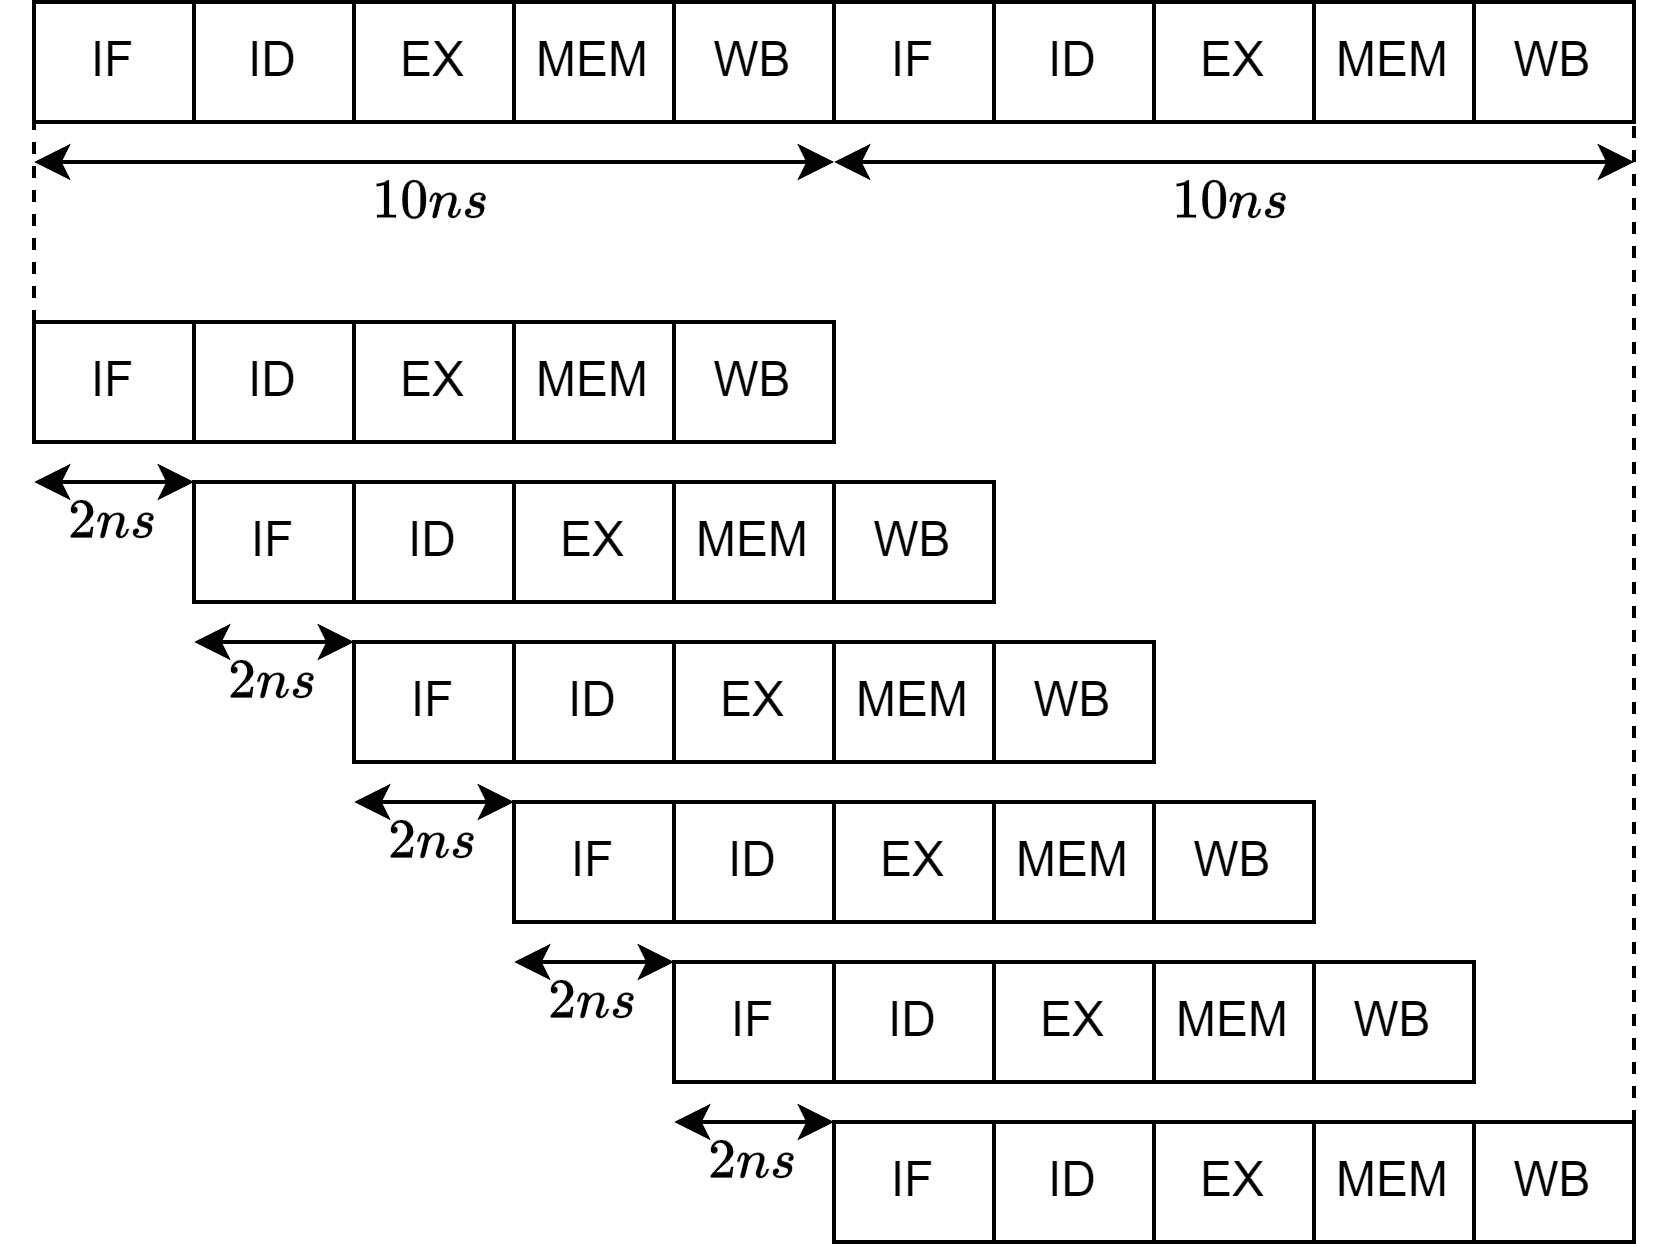
\includegraphics[width=0.5\linewidth]{images/exe.png}
    \caption{Sequential execution and pipelining execution}
\end{figure}

In pipelining, each stage of the pipeline corresponds to the time required to advance an instruction by one clock cycle. 
It's crucial to synchronize the pipeline stages, with the duration of a clock cycle determined by the slower stage of the pipeline, typically $2 ns$.

The objective is to achieve a balance in the length of each pipeline stage. When stages are perfectly balanced, the ideal speedup resulting from pipelining is equal to the number of pipeline stages. 
This ensures optimal utilization of the pipeline, enhancing overall performance and efficiency.

In the ideal scenario, we compare a single-cycle unpipelined CPU1 with a clock cycle of $8ns$ to a pipelined CPU2 with five stages of $2ns$ each. 
In this case the latency (total execution time) of each instruction is increased from $8ns$ to $10ns$ due to the pipeline overhead.
However, the throughput (number of instructions completed in a given time unit) is enhanced by four times: CPU1 completes one instruction every $8ns$, while CPU2 completes one instruction every $2ns$.

In the ideal scenario, when comparing a multi-cycle unpipelined CPU3 consisting of five cycles of $2ns$ each to a pipelined CPU2 with five stages of $2ns$ each. 
The latency (total execution time) of each instruction remains constant at $10ns$.
However, the throughput (number of instructions completed in a given time unit) is enhanced by five times: CPU3 completes one instruction every $10ns$, while CPU2 completes one instruction every $2ns$.

\subsection{Possible issues}
A potential concern arises due to the two-stage nature of the register file: read access during the instruction decode stage and write access during the write-back stage.
When a read and a write operation target the same register within the same clock cycle, it necessitates the insertion of a stall to prevent issues.

\begin{definition}[\textit{Optimized pipeline}]
    An optimized pipeline is achieved when the register file read operation takes place in the second half of the clock cycle, while the register file write operation occurs in the first half of the clock cycle.
\end{definition}

Another potential issue is the occurrence of hazards within the pipeline.
Hazards arise when there is a dependency between instructions, and the pipelining process causes a change in the order of accessing operands involved in the dependency, thereby preventing the next instruction from executing during its designated clock cycle.
Hazards diminish the performance from the ideal speedup achieved by pipelining.
Hazards can be categorized into three main types:
\begin{itemize}
    \item \textit{Structural hazards}: these occur when different instructions attempt to use the same resource simultaneously. 
        For example, there may be a conflict when both instructions require access to a single memory unit for instructions and data.
    \item \textit{Data hazards}: these occur when an instruction tries to use a result before it is ready. 
        For instance, an instruction might depend on the result of a previous instruction that is still in the pipeline.
    \item \textit{Control hazards}: these occur when a decision regarding the next instruction to execute is made before the condition for the decision is evaluated. 
        For instance, issues arise during conditional branch execution.
\end{itemize}
If dependent instructions are executed closely within the pipeline, data hazards become more prevalent.

\subsection{Data hazards}
\paragraph*{Read after write}
A data hazard of the "read after write" type occurs when an instruction $j$ attempts to read an operand before instruction $i$ has written to it. This hazard, known as a "dependence" in compiler terminology, arises from a genuine necessity for communication between instructions.
The potential solutions for mitigating this hazard include:
\begin{itemize}
    \item \textit{Compilation techniques}: 
        \begin{itemize}
            \item Insertion of "nop" (no operation) instructions.
            \item Instruction scheduling: the compiler arranges instructions to ensure that dependent instructions are not placed too close together. 
                It attempts to intersperse independent instructions among dependent ones. 
                If independent instructions cannot be found, the compiler inserts "nop" instructions.
        \end{itemize}
    \item \textit{Hardware techniques}:
        \begin{itemize}
            \item Insertion of "bubbles" or stalls in the pipeline.
            \item Data Forwarding or Bypassing: this technique involves using temporary results stored in the pipeline registers instead of waiting for the results to be written back to the register file. 
                Multiplexers are added at the inputs of the ALU to fetch inputs from pipeline registers, thus avoiding the need to insert stalls in the pipeline.
        \end{itemize}
\end{itemize}
Utilizing forwarding allows for resolving this conflict without introducing stalls in most cases. 
However, for load/use hazards, it is imperative to insert one stall to properly address the issue.

\paragraph*{Write after write}
A data hazard of the "write after write" type arises when instruction $j$ writes operand before instruction $i$ writes it. 
This situation results in write operations being executed in an incorrect order. 
Notably, this type of hazard does not occur in the MIPS pipeline since all register write operations take place in the write-back stage. 
Compiler writers classify this hazard as an output dependence.

\paragraph*{Write after read}
A data hazard of the "write after write" type arises when an instruction $j$ writes operand before instruction $i$ reads it. 
This scenario leads to the possibility of reading an incorrect value. However, such hazards do not occur in the MIPS pipeline because operand read operations take place in the instruction decode stage, while write operations occur in the write-back stage.
Similarly, assuming that register writes in ALU instructions occur in the fourth stage and that two stages are needed to access the data memory, some instructions might read operands too late in the pipeline.
Compiler writers classify this hazard as an anti-dependence.